\documentclass[12pt]{beamer}
\usepackage{amsmath}
\usepackage[utf8]{inputenc}
\usepackage{apacite}
\usetheme{Singapore}
\usepackage[style=british]{csquotes}

\def\signed #1{{\leavevmode\unskip\nobreak\hfil\penalty50\hskip1em
		\hbox{}\nobreak\hfill #1
		\parfillskip=0pt \finalhyphendemerits=0 \endgraf}}

\newsavebox\mybox
\newenvironment{aquote}[1]
{\savebox\mybox{#1}\begin{quote}\openautoquote\hspace*{-.7ex}}
	{\unskip\closeautoquote\vspace*{1mm}\signed{\usebox\mybox}\end{quote}}

\DeclareMathOperator*{\argmin}{arg\,min}
\usepackage{soul}

\title{Factor Strength and Factor Selection}
\subtitle{An Application to U.S. Stock Market}
\date{\today}
\author[author]{Zhiyuan Jiang\\
			                    28710967\\
			                    [10mm]
			                    {\small Supervisors: Dr Natalia Bailey 
			                    	\\ \hspace{18.5mm} 
			                    	Dr David Frazier}}
		
		
\begin{document}
	
\frame{\titlepage}

%-------------------------------------------------------------------------------------------------------------------------------------------------------------------------------%
%-------------------------------------------------------------------------------------------------------------------------------------------------------------------------------%
\section{Introduction and Motivation}

\begin{frame}{Introduction and Motivation}
Capital Asset Pricing Model (CAPM) is the benchmark of risk pricing.
\[r_{it} - r_{ft} = a_i + \beta_{im}(r_{mt} - r_{ft}) + \sum_{j=1}^{k}\beta_{ij}f_{jt} + \varepsilon_{it} \]

\frametitle{Motivation}
\begin{columns}
	\begin{column}{0.5\textwidth}
\begin{itemize}
\item $r_{it}$: asset's return
\item $r_{ft}$: risk free return
\item $a_i$: constant/intercept
\item $\beta_{im}$: market factor loading
\end{itemize}
	\end{column}
	\begin{column}{0.5\textwidth}  
		\begin{center}
\begin{itemize}
\item $r_{mt}$: market return 
\item$\beta_{ij}$: risk factor loading
\item $f_{jt}$: risk factor
\item $\varepsilon_{it}$: stochastic error
\end{itemize}
		\end{center}
	\end{column}
\end{columns}
\begin{itemize}
\item{\bf Add factors to enhance risk pricing.}
\item{\bf  New factors are booming }
\end{itemize}
\end{frame}

\begin{frame}[plain]
	\begin{figure}
\includegraphics[scale = 0.5]{figure/factor_growth.png}
\caption{Factor amount growing through the year. }
	\cite{Harvey2019}\\
	\end{figure}
\end{frame}

\begin{frame}
\begin{aquote}{\citeNP{Cochrane2011}}
We have a lot of questions to answer: \\
Firstly, which characteristics really provide \textbf{independent} information about average returns? Which are subsumed by others ?
\end{aquote}
	\begin{figure}
	
\includegraphics[scale = 0.2]{figure/cochrane.png}
\end{figure}
\end{frame}

\begin{frame}{Core Problem}
\begin{center}
\alert{\textbf{How to select factors.}}\pause
\end{center}
Numerous research has been done...
\begin{itemize}
\item Solving data mining problem 
\item Bayes method
\item Machine learning
\item $\cdots$
\end{itemize}

\end{frame}


\begin{frame}
	\frametitle{Two Challenges}
	This project faces two challenges:
	\begin{enumerate}
		\item	 High dimensions of data group\\
		How to identify the significant one. $\Rightarrow$ \alert{use factor strength as criteria.}
		\item 	Correlation among factors \\
		Traditional variable selection algorithm (Lasso) can not handle this.$\Rightarrow$ Will use \alert{elastic net} techniques
	\end{enumerate}
\end{frame}



%-------------------------------------------------------------------------------------------------------------------------------------------------------------------------------%
%-------------------------------------------------------------------------------------------------------------------------------------------------------------------------------%


	\section{Data and Methodology}
	
	\begin{frame}
		\frametitle{Data}
		The data set included two parts:
		\begin{itemize}
			\item {\bf Assets}: Standard \& Poor (S\&P) 500 index companies, three year U.S. t-bill, and average market return.\\
			\item {\bf Factor}:  145 factors plus one market factor \\

\item \textbf{Time period}:	Collect thirty years data: 1988:1-2017:12.\\

\item 		Divided into three subsamples: 10/20/30 years.\\
\end{itemize}		
		\resizebox{\textwidth}{!}{	\begin{tabular}{c|ccc}
				\hline
				& Time Span                    & Number of Companies (n) & Observations Amount (T) \\ \hline
				10 Years & January 2008 - December 2017 & 419                  & 120                     \\
				20 Years & January 1998 - December 2017 & 342                  & 240                     \\
				30 Years & January 1988 - December 2017 & 242                  & 360                     \\ \hline
		\end{tabular}}
	\end{frame}
	
	\begin{frame}
		\frametitle{Factor Strength}
		Strong factor $\Rightarrow$ price more asset's risk $\Rightarrow$ generate more significantly loadings $\beta$.\\
		Factor strength is defined in terms of factor loading \cite{Bailey2020}.\\
		
		 Assume we have N different assets.
		\begin{align*}
		|\beta_j| &> 0,\quad j = 1, 2, 3, \cdots, [N^{\alpha_j}]\\
		|\beta_j |&= 0, \quad j = [N^{\alpha_j} ]+1 ,[N^{\alpha_j}]  +2, [N^{\alpha_j}] +3, \cdots, N
		\end{align*}
	
Simply speaking: the more none-zero loadings a factor can generate, the stronger the factor is.
	\end{frame}

\begin{frame}
	For every single risk factor, after running a bunch of regression against different assets, we will have a proportion:\\
 Proportion	$\hat{\pi_n}$, represent how many non-zero significant loadings are generated.\\
\[\hat{\alpha}_{j}=\left\{\begin{array}{l}
	1+\frac{\ln \hat{\pi}_{n T, j}}{\ln n}, \text { if } \hat{\pi}_{n T, j}>0 \\
	0, \text { if } \hat{\pi}_{n T, j}=0
\end{array}\right.\]

$\alpha \in [0,1]$.\\
0 means no loadings are generate, and 1 means the factor can generate loadings to every assets.
\end{frame}

	
\begin{frame}
\frametitle{Elastic Net}
Introduce by \citeA{Zou2005}, is a improved method to select factor.

Considering the following loss function:

	\[   \hat{\beta}_{ij}  = \argmin_{\beta_{ij}}\{\sum_{i = 1}^{n}[(r_{it} - r_{ft}) - \beta_{ij }f_{jt}]^2 + \lambda_2\sum_{i = 1}^{n}\beta_{ij}^2  + \lambda_1\sum_{i = 1}^{n}|\beta_{ij}|     \}    \]
	
	The $L_1$ norm $\sum_{i = 1}^{n}|\beta_{ij}|$ helps select the factor, reduce redundancy.\\
    The $L_2$ norm $\sum_{i = 1}^{n}\beta_{ij}^2 $ helps handle the correlation.

\end{frame}

\begin{frame}
	\frametitle{Elastic Net: In empirical}
We use R package \textbf{\textit{glmnet}}, and the package using loss function \cite{Friedman2010}:
	
\[	\boldsymbol{\hat{\beta}}_{i} = \argmin \{ \frac{1}{2N} (x_{it}-\hat{a}_{iT} - \boldsymbol{\hat{\beta}_{i}^{\prime}f_t}^2 ) +\phi P_{\theta}(\boldsymbol{\beta_i})  \} \]

\[	P_{\theta}(\boldsymbol{\beta_i}) =\sum_{j=1}^k [ (1-\theta)\boldsymbol{\beta}_{ij}^2 + \theta |\boldsymbol{\beta}_{ij}|] \]\\
We have to decide two parameter: $\phi$, and $\theta$.

\end{frame}


\section{Empirical Findings}

\begin{frame}[plain]
		\frametitle{Proportion of Strength (145 risk factors)}
\begin{figure}
        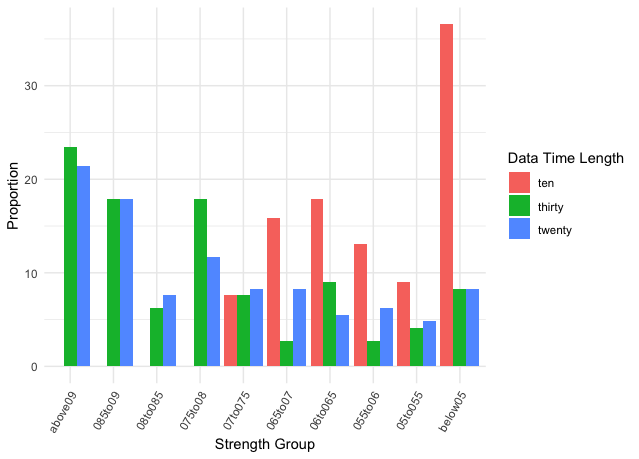
\includegraphics[scale = 0.5]{figure/strength_proportion.png}
\end{figure}
\end{frame}


\begin{frame}
	\frametitle{Top 10 strong factors and three famous factors}
\resizebox{\textwidth}{!}{
	\begin{tabular}{llc|llc|llc}
	\hline
	\multicolumn{3}{c|}{Ten Year} & \multicolumn{3}{c|}{Twenty Yera} & \multicolumn{3}{c}{Thirty Year} \\ \hline
	Rank & Factor     & Strength & Rank   & Factor     & Strength   & Rank   & Factor     & Strength   \\ \hline
	 	 & Market & 0.988 & &Market & 0.990 & &Market & 0.995 \\
	1   & beta               & 0.749    & 1      & ndp           & 0.937      & 1      & salecash  & 0.948\\
	2   & baspread       & 0.730    & 2      & quick        & 0.934      & 2      & ndp          & 0.941\\
	3   & turn               & 0.728    & 3      & salecash   & 0.933      & 3      & quick      & 0.940\\
	4   & zerotrade      & 0.725    & 4      & lev            & 0.931      & 4      & age         & 0.940\\
	5   & idiovol           & 0.723    & 5      & cash         & 0.931      & 5      & roavol    & 0.938\\
	6   & retvol            & 0.721    & 6      & dy             & 0.929      & 6      & ep           & 0.937\\
	7   & std\_turn      & 0.719    & 7      & roavol      & 0.929      & 7      & depr       & 0.935\\
	8   & HML\_Devil & 0.719    & 8      & zs              & 0.927      & 8      & cash       & 0.934\\
	9   & maret           & 0.715    & 9        & age          & 0.927      & 9      & rds         & 0.931\\
	10 & roavol          & 0.713    & 10     & cp             & 0.926      & 10    & dy          & 0.927 \\
	20 & UMD            & 0.678    & 29     & HML        & 0.905      & 39     & HML       & 0.894 \\
	24 & HML            & 0.672    & 76     & SMB        & 0.770      & 68     & SMB        & 0.804 \\
	87 & SMB            & 0.512    & 89     & UMD        & 0.733      & 96     & UMD       & 0.745 \\ 
	\hline
\end{tabular}
}
\end{frame}


\begin{frame}[plain]
	\frametitle{Correlation of Factors: from strong to weak}
	\begin{figure}
		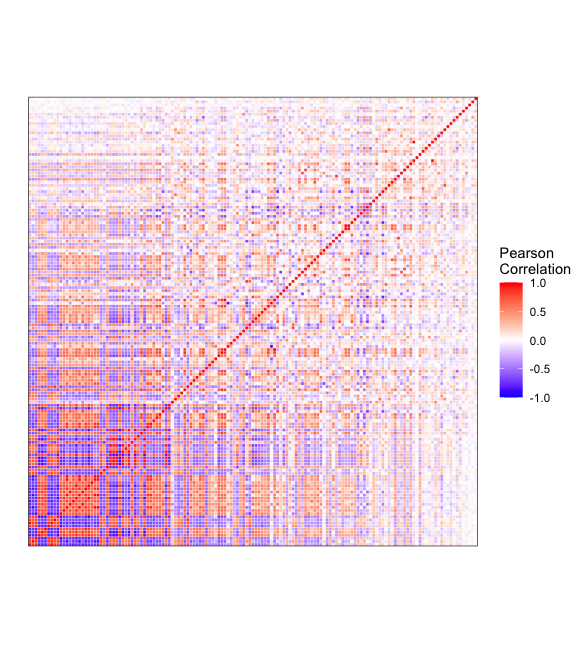
\includegraphics[scale = 0.4]{figure/correlation_heat_map.png}
	\end{figure}
\end{frame}


\begin{frame}
\frametitle{Correlation among factors.}
\resizebox{\textwidth}{!}{
	\begin{tabular}{l|cccccc}
		\hline
		\hline
		Factor Group                                 & (0,0.5{]} & (0.5, 0.6{]} & (0.6, 0.7{]} & (0.7, 0.8{]} & (0.8,0.9{]} & (0.9,1{]} \\ \hline
		\multicolumn{1}{c|}{Correlation Coefficient} & 0.0952    & 0.157        & 0.213        & 0.229        & 0.371       & 0.724   \\
		Factor Amount &12 & 10 &  17 & 37& 35 &34  \\ \hline \hline
	\end{tabular}\\
}\\

\begin{itemize}
\item Correlation among strong factor is very high.
\item Among weak factors is very low.
\item  Recall the correlation problem Lasso can not handle...
\end{itemize}

\end{frame}



\begin{frame}
	\frametitle{Factor Selection Result}
	\resizebox{\textwidth}{!}{

			\begin{tabular}{l|ccccccc}
			\hline
			\hline
Factor Group                                     & (0,0.5] & (0.5, 0.6] & (0.6, 0.7] & (0.7, 0.8] & (0.8,0.9] & (0.9,1] & Mix    \\ 
			Factor Amount                  & 12            & 10               & 17               & 37               & 35              & 34            & 20  \\ \hline
			\begin{tabular}[c]{@{}c@{}}Proportion of Agreement\\ (Exact)\end{tabular} & 68.7\%                        & 55.9\%                           & 42.8\%                           & 20.9\%                           & 17.7\%                          & 13.9\%                        & 34.6\% \\
			\begin{tabular}[c]{@{}c@{}}Proportion of Agreement\\ (90\%)\end{tabular}  & 86.8\%                        & 72.0\%                           & 74.5\%                           & 72.0\%                           & 79.8\%                          & 74.4\%                        & 76.1\% \\\hline
		Avg EN selection amount        & 2.11          & 4.47             & 8.67             & 14.67            & 13.51           & 12.37         & 8.45                  \\
		Avg EN selection proportion    & 17.5\%        & 44.73\%          & 51.00\%          & 39.65\%          & 38.61\%         & 36.38\%       & 42.28\%                 \\
		Avg Lasso selection amount     & 2.06          & 3.87             & 8.43             & 13               & 12.19           & 10.46         & 7.26                    \\
		Avg Lasso selection proportion & 17.2\%        & 38.76\%          & 49.60\%          & 35.14\%          & 34.83\%         & 30.75\%       & 36.27\%                 \\ \hline\hline
	\end{tabular}
}
\begin{itemize}
\item Agreement decrease with factor strength increase
\subitem	May because of the correlation
\item	Lasso produce parsimonious model
\item	When facing weak factors, both Lasso and EN can well reduce redundancy.
\subitem Eight of Top 10 most selected factors from mix factor group are strong factors.
\end{itemize}
\end{frame}

%-------------------------------------------------------------------------------------------------------------------------------------------------------------------------------%
%-------------------------------------------------------------------------------------------------------------------------------------------------------------------------------%


\section*{epilogue}
\begin{frame}
\frametitle{Potential Extension}
\begin{enumerate}
\item Using other criterion for tuning parameter
\item Categorised the factors and stocks
\item Using other methods to select factors, compare with the Lasso and Elastic net.
\end{enumerate}
\end{frame}


\begin{frame}
	\centering	
\huge{ Thanks for listening\\}
\end{frame}

	\section*{}
\begin{frame}
\frametitle{EN parameter tuning}
\[	\boldsymbol{\hat{\beta}}_{i} = \argmin \{ \frac{1}{2N} (x_{it}-\hat{a}_{iT} - \boldsymbol{\hat{\beta}_{i}^{\prime}f_t}^2 ) +\phi P_{\theta}(\boldsymbol{\beta_i})  \} \]

\[	P_{\theta}(\boldsymbol{\beta_i}) =\sum_{j=1}^k [ (1-\theta)\boldsymbol{\beta}_{ij}^2 + \theta |\boldsymbol{\beta}_{ij}|] \] \\
The R package \textit{glmnet} provides function to tuning parameter $\phi$, using cross-validation, targeting at minimise the MSE.\\
We use the same principle: minimise the MSE to determine our $\theta$ value.\\
\end{frame}

	\section*{}
\begin{frame}
Assume we have n units of stock, j risk factors, and t observations.\\
\begin{enumerate}
\item Assign first 90\% of data as learning set, and rest 10\% as test set.
\item Prepare a sequence of $\theta$ values, from 0 to 1, with step 0.01
\item For each $\theta$, we use the learning set to fit a model, with $\phi$ selected by the function
\item Base on the fitted model, makes prediction and compare with the test set, and calculate the MSE.
\item The $\theta-\phi$ combination with smallest MSE is the winner.
\end{enumerate}
\end{frame}

%-------------------------------------------------------------------------------------------------------------------------------------------------------------------------------%
%-------------------------------------------------------------------------------------------------------------------------------------------------------------------------------%
\begin{frame}[allowframebreaks]
	\frametitle{Bibliography}
	\bibliographystyle{apacite}
{\footnotesize\bibliography{library.bib}}
\end{frame}
\end{document}